\documentclass[12pt, a4paper]{article}
\usepackage{fullpage}
\usepackage{graphicx}
\usepackage{amsmath}
\usepackage{amssymb}
\usepackage[hidelinks]{hyperref}
\usepackage{listings}
\usepackage{epigraph}
\renewcommand{\epigraphsize}{\footnotesize}
\setlength{\epigraphwidth}{.5\textwidth}
\lstset{
  language = C,
  basicstyle = \ttfamily \small,
  numbers = left,
  numberstyle = \footnotesize,
  showstringspaces = false
}
\usepackage{times}

\title{601 Comprehensive II}
\author{Jeremy Kong}
\date{18 June 2017}

\begin{document}
\maketitle

\noindent A couple of quick notes:
\begin{itemize}
\item I'd intend for the timelimit for this paper to be 3 hours and 20 minutes (200 minutes total).
\item This question was constructed by a student at Imperial College London, and is not intended to be representative of actual examination questions for any specific course at Imperial.
\item The material students have learned from the compulsory modules in first and second year should be sufficient to answer all questions.
\item Each question is worth 20 marks; the maximum mark is thus 100.
\item The questions are roughly arranged in what I think is difficulty order. Also, \textit{within each question} the difficulty generally increases as you progress from one part to the next.
\item This exam is \textbf{hard} and intended to be hard. The author obtained an average of $92.9$ percent in his second year at Imperial, but would only expect to score about $70$ on this exam.
\end{itemize}

\newpage
$\:$
\newpage 

\section{To A Brighter Day}
\epigraph{Cause if we lost our minds, and we took it way too far \\
I know we'd be alright, I know we would be alright \\
If you were by my side, and we stumbled in the dark \\
I know we'd be alright, I know we would be alright --
}{\textit{``There's Nothing Holding Me Back", Shawn Mendes}}
\begin{center}
\textbf{WARNING!}

This is the final question and is (in the author's opinion) the hardest. Good luck!
\end{center}

\noindent \textsc{Light Up} (also called \textsc{Akari}) is a logic puzzle first published 
by Nikoli \cite{lightup}. The puzzle is played on a two-dimensional plane and involves an 
$n \times n$ matrix of cells. An example of a \textit{very} simple puzzle and its solution
are shown below:
\begin{center}
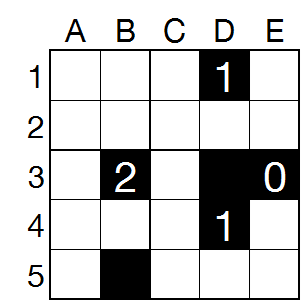
\includegraphics[scale=0.7]{lightsout1.png}
\hspace{3cm}
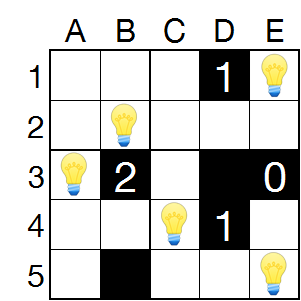
\includegraphics[scale=0.7]{lightsout2.png}
\end{center}

Players seek to place lightbulbs on some squares, subject to the following constraints:
\begin{itemize}
\item A lightbulb emits light in the four cardinal directions (north, south, east
and west). Light travels in a straight line until it hits a block (black square), or
the edge of the grid.
\item Lightbulbs can only be placed in white squares. They must light up all white squares
in the grid. The square a lightbulb itself is on is considered to be lit.
\item Lightbulbs must \textit{not} shine on each other. (However, a single square 
can be illuminated by multiple lightbulbs, as long as the bulbs
themselves don't light each other.)
\item Some black squares are marked with \textit{clues}. A clue indicates the number of
lightbulbs adjacent to the relevant black square (but \textit{only} in the four cardinal
directions).
\end{itemize}

For example, the simple puzzle above may be solved using the following reasoning.
\begin{itemize}
\item Neither E2 or E4 can contain a lightbulb (because of the 0 in E3).
\item The entire grid must be lit -- so E5 must contain a lightbulb, as must E1.
\item C1 and D2 cannot contain lightbulbs (because of the 1 in D1). Also, C5 and D5
cannot contain lightbulbs (because the bulb on E5 shines there). So C4 must have a lightbulb to satisfy the 1 in D4.
\item This means C3 and B4 cannot contain lightbulbs; but to satisfy the 2 in B3,
A3 and B2 must contain lightbulbs. We've now lit every square, so we are done.
\end{itemize}

\noindent In this question, we will walk through a proof that solving a \textsc{Light Up}
puzzle is, in the general case, extremely difficult (well, assuming that 
$\textsc{P} \neq \textsc{NP}$). Strictly speaking, the statement ``solving a \textsc{Light 
Up} puzzle is $\textsc{NP}$-complete" is bogus, because a \textsc{Light Up} puzzle is not 
a decision problem. We thus consider the decision problem \textsc{Light Up (D)}:

\begin{quote}
Given a \textsc{Light Up} puzzle, does a solution exist?
\end{quote}

\begin{enumerate}
\item Show that \textsc{Light Up (D)} is in NP.

\item We can show that \textsc{Light Up (D)} is NP-hard, by reducing the problem
\textsc{Circuit-Sat} to \textsc{Light Up (D)} \cite{akari2}. Recall the definition
of \textsc{Circuit-Sat}:

\begin{quote}
Given a boolean combinational circuit composed of AND, OR and NOT gates with a single
output, does there exist a truth assignment to its inputs such that the output is 
satisfied?
\end{quote}

In practice, this involves implementing a Boolean circuit using the constructs of the 
\textsc{Light Up} puzzle, and ensuring that our puzzle has a solution if and only if
the Boolean circuit

For example, we can use the presence or absence of a bulb to indicate a 1 or 0 signal
respectively. If we do this, we can implement a ``wire" as a corridor:

\begin{center}
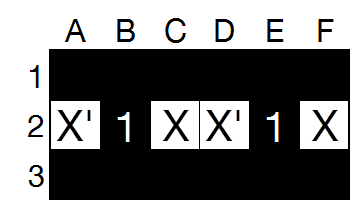
\includegraphics[scale=0.7]{lightsout3.png}
\end{center}

We define the state of a wire to be ``true" if we place bulbs in the cells marked with
$X$, and ``false" if we place bulbs in the cells marked with $X'$.

\begin{enumerate}
\item We may need to support a turn in the aforementioned corridors, to channel
our Boolean values around and supply them as input and output to our various gates.

Consider the following partially-filled in grid (note that this is not a
puzzle!).
\begin{center}
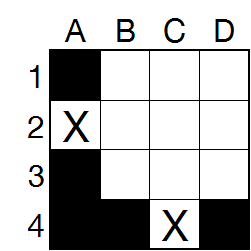
\includegraphics[scale=0.7]{lightsout4.png}
\end{center}

By shading some cells and adding clues where appropriate, demonstrate that it is possible
to create a puzzle where A2 contains a lightbulb \textit{if and only if} C4 contains
a lightbulb.

\item Describe how you might use the constructs in \textsc{Light Up} to model the
\textit{output} of the Boolean circuit in \textsc{Circuit-Sat}.

\item Consider the following Boolean circuit component, which takes two inputs $X$ and $Y$
and returns a single output $Z$. (Note that we have stretched the wires here, and
indicated $X'$ and $Y'$ as a reminder that although our inputs might be $X$ and $Y$,
the incident squares will have a bulb if and only if $X$ and $Y$ respectively are 
\textit{false}).

\begin{center}
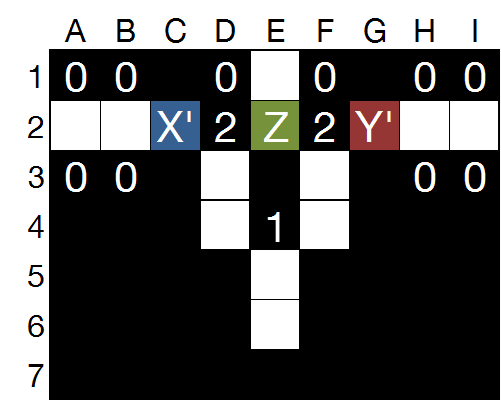
\includegraphics[scale=0.7]{lightsout5.png}
\end{center}

Express $Z$ as a function of $X$ and $Y$. Explain why $Z$ \textit{must} take on the
value of said function.

\item Complete the reduction, extending on your work in parts (a), (b) and (c).

(\textit{Hint}: It will be important to show that your puzzle design can handle
nonplanar ``channels". You may use without proof that wire crossing can be implemented
if you are able to fork the input and perform an XOR operation (because of the
well-known ``XOR in-place swap algorithm"). However, you need to supply the 
implementations of these yourself.)

\end{enumerate}

\item Show that, under the assumption $\textsc{P} \neq \textsc{NP}$, \textsc{Light Up}
in general cannot be solved in polynomial time.
\item Suppose you have a polynomial time algorithm to solve an NP-complete problem
(such as \textsc{Circuit-Sat} as introduced above). Present a polynomial time algorithm to 
solve \textsc{Light Up}. To be clear:
\begin{itemize}
\item Your algorithm should solve a \textsc{Light Up} puzzle -- \textit{not} answer the
decision version of the problem.
\item You may use without proof that the composition of two polynomials is polynomial.
\end{itemize}

\textit{The mark weighting for this question is as follows: 2, [1, 1, 4, 7], 1, 4, for a total of 20.}

\end{enumerate}

\newpage
\begin{thebibliography}{9}
\bibitem{lightup}
``Rules of Akari puzzle." Accessed 18 June 2017. $<$\url{http://www.nikoli.com/en/puzzles/bijutsukan/rule.html}$>$

\bibitem{akari2}
``Light Up is NP-complete." Accessed 18 June 2017. $<$\url{http://www.mountainvistasoft.com/docs/lightup-is-np-complete.pdf}$>$

\bibitem{orleans}
Bernstein, Philip A., et al. ``Orleans: Distributed Virtual Actors for Programmability and Scalability."
\end{thebibliography}

\newpage

\end{document}